\documentclass{article}

\usepackage[OT1]{fontenc}
\usepackage{amsmath}
\usepackage[utf8]{inputenc}
\usepackage{amssymb}
\usepackage{amsxtra}
\usepackage{listings}
\usepackage{graphicx}
\usepackage[dvipsnames]{xcolor}
\usepackage{tikz,lipsum,lmodern}
\usepackage[most]{tcolorbox}

\renewcommand*\familydefault{\sfdefault} % Set font to sans-serif
\graphicspath{ {figures/} }

\definecolor{highlight}{RGB}{29, 141, 176}

\newcommand{\refchapter}[1]{Chapter~\ref{#1}}
\newcommand{\refsec}[1]{Section~\ref{#1}}
\newcommand{\refeqn}[1]{Equation~(\ref{#1})}
\newcommand{\reffig}[1]{Figure~\ref{#1}}

\newenvironment{task}[1]{
  \begin{tcolorbox}[
    colback=highlight!5!white,
    colframe=highlight,
    title={Task #1}
  ]
}{
  \end{tcolorbox}
}

\title{
  \vspace*{2cm}
  {\bf \scriptsize
    KATHOLIEKE UNIVERSITEIT LEUVEN \\\vspace{0.3cm}
    Prof. Dr. ir. Johan A. K. Suykens
  } \vspace{2cm} \\
  Artificial Neural Networks \& Deep Learning \\
  {\large Exercise Reports}
}
\author{Marco Bischoff (R1012984)}

\begin{document}


\pagestyle{headings}

\maketitle
\newpage

\tableofcontents
\newpage



\section{Supervised Learning and Generalization}
\label{ex:1}

\setcounter{subsection}{2}
\subsection{In the Wide Jungle of the Training}
\label{task:1.3}


\begin{task}{1.3.1}
  What is the impact of the noise (parameter \texttt{noise} in the notebook) with respect to the
  optimization process?
\end{task}

The noise parameter controls the deviation of the training data from the true function.
Figure~\ref{fig:ex1_noise-level} shows the impact of noise on the optimization process. For $noise =
  0$, the data exactly matches the true function and the model will converge to the true function
quickly. For $noise > 0$, the data is perturbed by noise and the model will take longer to converge.
For $noise = 1$, the data is completely random and the model will only converge to the mean of the
training data without being able to capture the underlying function.
\begin{figure}[ht!]
  \centering
  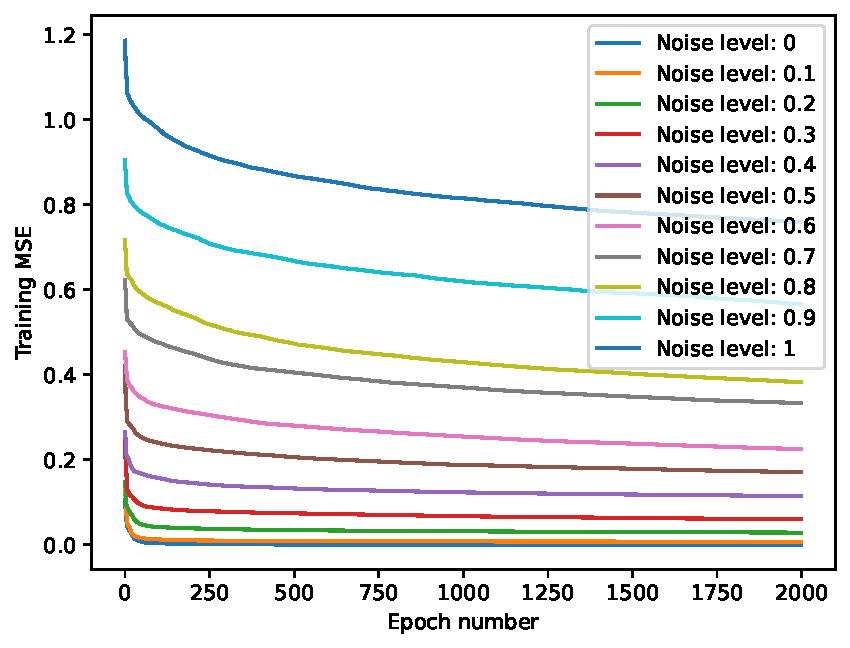
\includegraphics[width=0.8\textwidth]{ex1_noise-level.pdf}
  \caption{Impact of noise on the optimization process}
  \label{fig:ex1_noise-level}
\end{figure}


\begin{task}{1.3.2}
  How does (vanilla) gradient descent compare with respect to its stochastic and accelerated
  versions?
\end{task}

Vanilla gradient descent is the slowest of the three methods. It computes the gradient of the loss
function for the entire training set at each iteration. Stochastic gradient descent (SGD) is faster
than vanilla gradient descent, because it computes the gradient for a random subset of the training
data at each iteration. However it has a higher variance in the loss function. Accelerated gradient
descent is the fastest of the three methods. It uses a momentum term to speed up convergence and
reduce oscillations in the loss function.


\begin{task}{1.3.3}
  How does the size of the network impact the choice of the optimizer?
\end{task}

For small networks, vanilla gradient descent is sufficient, because the computation of the gradient
is not very expensive. For larger networks, SGD is more appropriate due to its lower computational
cost. Accelerated gradient descent is the best choice for very large networks, because it converges
faster than the other two methods.


\begin{task}{1.3.4}
  Discuss the difference between epochs and time to assess the speed of the algorithms. What can it
  mean to converge fast?
\end{task}

The model is trained for $2500$ epochs. In Figure~\ref{fig:ex1_optimizers}, we can see that SGD with
a learning rate of $0.05$ and without momentum has an average training time, but very slow
convergence. Using a learning rate of $0.1$ already converges much faster, but also takes longer to
compute. Momentum has a similar convergence rate and is much quicker to compute, but also has high
variance. The Adam and the LBFGS optimizers converge the fastest, but LBFGS has the longest
computational time. The Adam optimizer is the best choice for this problem, because it converges
quickly and has low variance. All optimizers except for vanilla SGD with learning rate $0.05$ can
be considered to have converged after at most $1000$ epochs.
\begin{figure}[ht!]
  \centering
  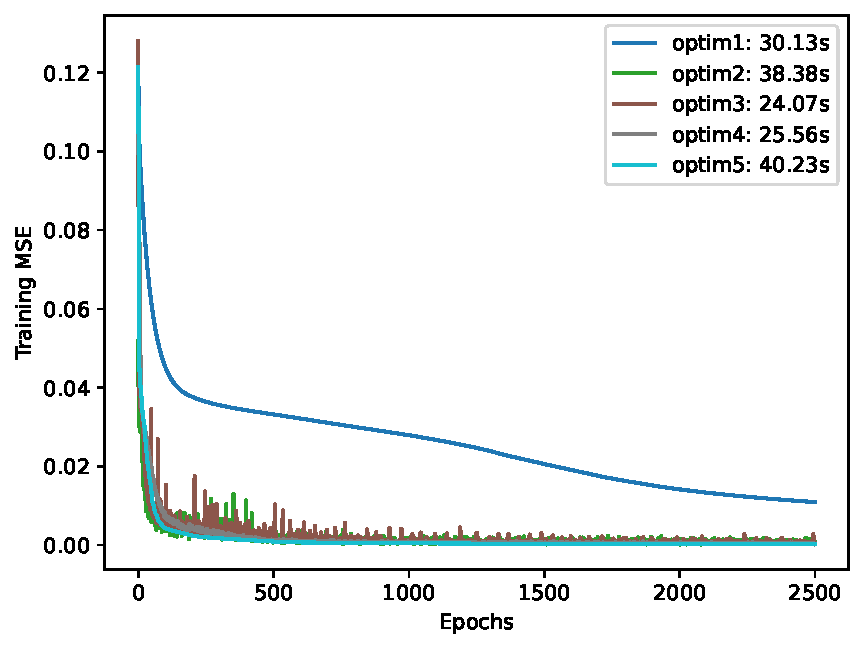
\includegraphics[width=0.8\textwidth]{ex1_optimizers.pdf}
  \caption{Comparison of optimizers}
  \label{fig:ex1_optimizers}
\end{figure}


\subsubsection*{A bigger model}
\begin{task}{1.3.5}
  How many parameters does the model have?
\end{task}

The model has $34826$ parameters in total as shown in Table~\ref{tab:ex1_model}.

\begin{table}[ht!]
  \begin{tabular}{|l|l|r|}
    \hline
    \textbf{Layer Type} & \textbf{Output Shape} & \textbf{Number of Parameters} \\ \hline
    (Input)             & (28, 28, 1)           & 0                             \\ \hline
    Conv2D              & (26, 26, 32)          & 320                           \\ \hline
    MaxPooling2D        & (13, 13, 32)          & 0                             \\ \hline
    Conv2D              & (11, 11, 64)          & 18496                         \\ \hline
    MaxPooling2D        & (5, 5, 64)            & 0                             \\ \hline
    Flatten             & (1600, )              & 0                             \\ \hline
    Dropout             & (1600, )              & 0                             \\ \hline
    Dense               & (10, )                & 16010                         \\ \hline\hline
    \textbf{Total}      &                       & \textbf{34826}                \\ \hline
  \end{tabular}
  \centering
  \caption{Model parameters}
  \label{tab:ex1_model}
\end{table}


\begin{task}{1.3.6}
  Replace the ADAM optimizer by a SGD one. Can you still achieve excellent performances? Try then
  the Adadelta optimizer. What is its particularity?
\end{task}

The SGD optimizer has a much slower convergence rate than the Adam optimizer as shown in
Figure~\ref{fig:ex1_mnist_optimizers}. The Adadelta optimizer achieves almost perfect performance
after the first epoch and has a very low variance. The Adam optimizer is in between the two in terms
of convergence rate and variance.
\begin{figure}[ht!]
  \centering
  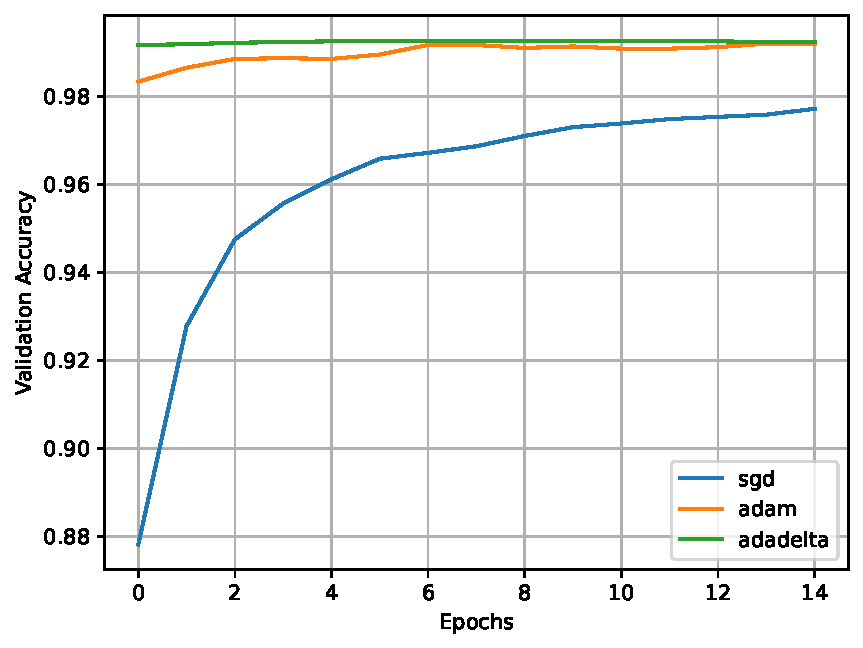
\includegraphics[width=0.8\textwidth]{ex1_mnist_optimizers.pdf}
  \caption{Validation accuracy}
  \label{fig:ex1_mnist_optimizers}
\end{figure}




%%%%%%%%%%%%%%%%%%%%%%%%%%%%%%%%%%%%%%%%%%%%%%%%%%%%%%%%%%%%%%%%%%%%%%%%%%%%%%%%%%%%%%%%%%%%%%%%%%%%

\cite{Ries1522Rad}

\newpage
\nocite{}
\bibliographystyle{plain}
\bibliography{main}



\appendix

\section{Benutzerdokumentation}
\label{app1}
\section{Introduction}


\end{document}

